\section{Resultados de experimentaci\'on}

El uso del software no se ve limitado a las personas con movilidad reducida,
 este le puede servir incluso a las personas que no tengan discapacidad 
 alguna, ya que no va por una tarea objetivo espec\'ifica, sino por las 
 actividades que realice la persona de forma frecuente sin importar cuales 
 sean. Con esto en mente, se logr\'o obtener 5 archivos con la lista de 
 acciones que realizaron 4 individuos sin discapacidades y un quinto con 
 discapacidad en brazos o manos en sus actividades cotidianas en una 
 computadora


En el periodo de aproximadamente 4 meses comprendido del 24/02/2018 al 
 30/06/2018 para las primeras 4 personas, mientras que, la persona 
 condiscapacidad solo uso la computadora durante 6 dias. Durante estos 
 periodos las personas tuvieron encendida su computadora diferente cantidad 
 de tiempo el cual se muestra en la segunda columna de la tabla 
 \ref{infodata}. Como ya se explic\'o anteriormente en el cap\'itulo 
 \ref{sec:chapter4} una acci\'on realizada por el usuario genera un nodo, 
 esta cantidad es mostrada en la columna 3, mientras que la columna 4 es el 
 n\'umero m\'aximo de veces que se repiti\'o un nodo y para mantener el 
 anonimato de las personas participantes en esta prueba, se les har\'a 
 referencia por un n\'umero como se muestra en la primer columna. 

Se observa en la tabla \ref{infodata} que el sujeto \textbf{n\'umero 3}
 es el que tiene el mayor tiempo de uso con mas de 1060 horas, con
 1,448,016 nodos generados y 378,541 veces que se repiti\'o un nodo como 
 m\'aximo; mientras que el sujeto \textbf{n\'umero 1} con 1,494,792 nodos, es 
 el que obtuv\'o mayor cantidad de nodos reportados en 166 horas y 23 minutos 
 con 46,036 repeticiones de un nodo. Finalmente, el sujeto \textbf{n\'umero 
 5} tiene el menor tiempo con 17 horas y 56 minutos, con 281,794 nodos y 
 8,945 repeticiones reportadas.


\begin{table}[]
\centering
\scalebox{0.9}{
\begin{tabular}{cccc}
\hline
\textbf{No. de Sujeto}	
&   \textbf{Tiempo de Uso (Hr:Min)}		
&	\textbf{N\'umero de Nodos}
&   \textbf{Repeticiones} 	\\   
\hline

1				
&	166:23 						
&	1,494,792			
&	46,036				\\
		
2
&	490:24
&	1,333,016
&	116,001				\\
		
3
&	1060:48
&	1,448,016
&	378,541				\\
		
4
&	148:23
&	972,828
&	56,606				\\ 

5	
&	17:56
&	281,794
&	8,945				\\
\hline

\end{tabular}
}
\caption{Informaci\'on de los datos recabados.}
\label{infodata}
\end{table}

A cada lista de acciones se le aplic\'o el algoritmo explicado en el
 cap\'itulo \ref{sec:chapter4}, utilizando un factor de 70 incidencias, para 
 que el  nodo 
 sea candidato a formar una secuencia; ya que al utilizar un n\'umero menor, 
 se estar\'ian aceptando la  mayor\'ia de las acciones, lo cual representa un 
 menor tiempo para mostrar una tarea, pero m\'as secuencias basura que 
 tendr\'ia que depurar el usuario  manualmente y por el contrario si el 
 factor es mayor, la identificaci\'on de  secuencias ser\'ia lenta y con 
 algunas secuencias basura, y un m\'inimo de 5  repeticiones por secuencia 
 para declarar que la tarea es \'util. 


Las secuencias de acciones que empieza con la acci\'on \emph{Release} fueron 
 descartadas, ya que esta acci\'on implica que se qued\'o presionada una 
 tecla o bot\'on espec\'ifico; tambi\'en se rechazaron las que 
 terminen con la acci\'on \emph{Pressed} ya que esto dejar\'ia presionada la 
 tecla o bot\'on hasta que se presione f\'isicamente o se mande a llamar la 
 acci\'on \emph{Release}, 
 por ejemplo, una de la tareas que se ver\'ian afectadas por las limitantes
 mencionadas, podr\'ia ser el seleccionar varios iconos no consecutivos en 
 Windows, ya que una forma de hacerlo es mantener presionada(Pressed) la
 tecla CTRL y seleccionar los iconos con el rat\'on uno a uno dando clic 
 sobre ellos y posteriormente soltar(Release) la tecla CTRL, principalmente 
 por la falta de precisi\'on al mover el rat\'on, ya que estas variaciones 
 evitan que se genere una secuencia completa de la tarea, dejando la tecla 
 presionada.



En la figura \ref{fig:graphKB}, se presenta el grafo generado con las
 primeras 150 acciones del teclado del sujeto \textbf{n\'umero 3},
 mientras que en la figura \ref{fig:zoomKB} se hace la ampliaci\'on a un
 conjunto de nodos en los que se muestra la relaci\'on de  
 (\textsc{\char13}Keyboard\textsc{\char13},\textsc{\char13}Pressed
 \textsc{\char13},\textsc{\char13}Key.shift\_r\textsc{\char13}) en la parte 
 inferior central y el nodo (\textsc{\char13}Keyboard\textsc{\char13},
 \textsc{\char13}Release\textsc{\char13},\textsc{\char13}Key.shift\_r
 \textsc{\char13}) ubicado en la parte superior izquierda. En la figura 
 \ref{fig:morezKB} se Se muestra el acercamiento al nodo 
 (\textsc{\char13}Keyboard\textsc{\char13},\textsc{\char13}Pressed
 \textsc{\char13},\textsc{\char13}Key.shift\_r\textsc{\char13}),
 en esta se aprecia la relaci\'on con otros nodos, lo cual 
 implica que este nodo, es uno de los que mas se repite, dado que es utilizado
 en varias secuencias usadas por este usuario. 
 
En la siguiente direcci\'on web es posible encontrar el 
 grafo en formato PDF, para su mejor observaci\'on, as\'i como el 
 generado con las primeras 600 acciones del rat\'on por el mismo sujeto.
 
 
\begin{center}
 \url{https://1drv.ms/f/s!Ap61Bj4GJQX2iOppX2n1jChCHyxqdQ} 
\end{center}



\begin{figure}[h]
\centering
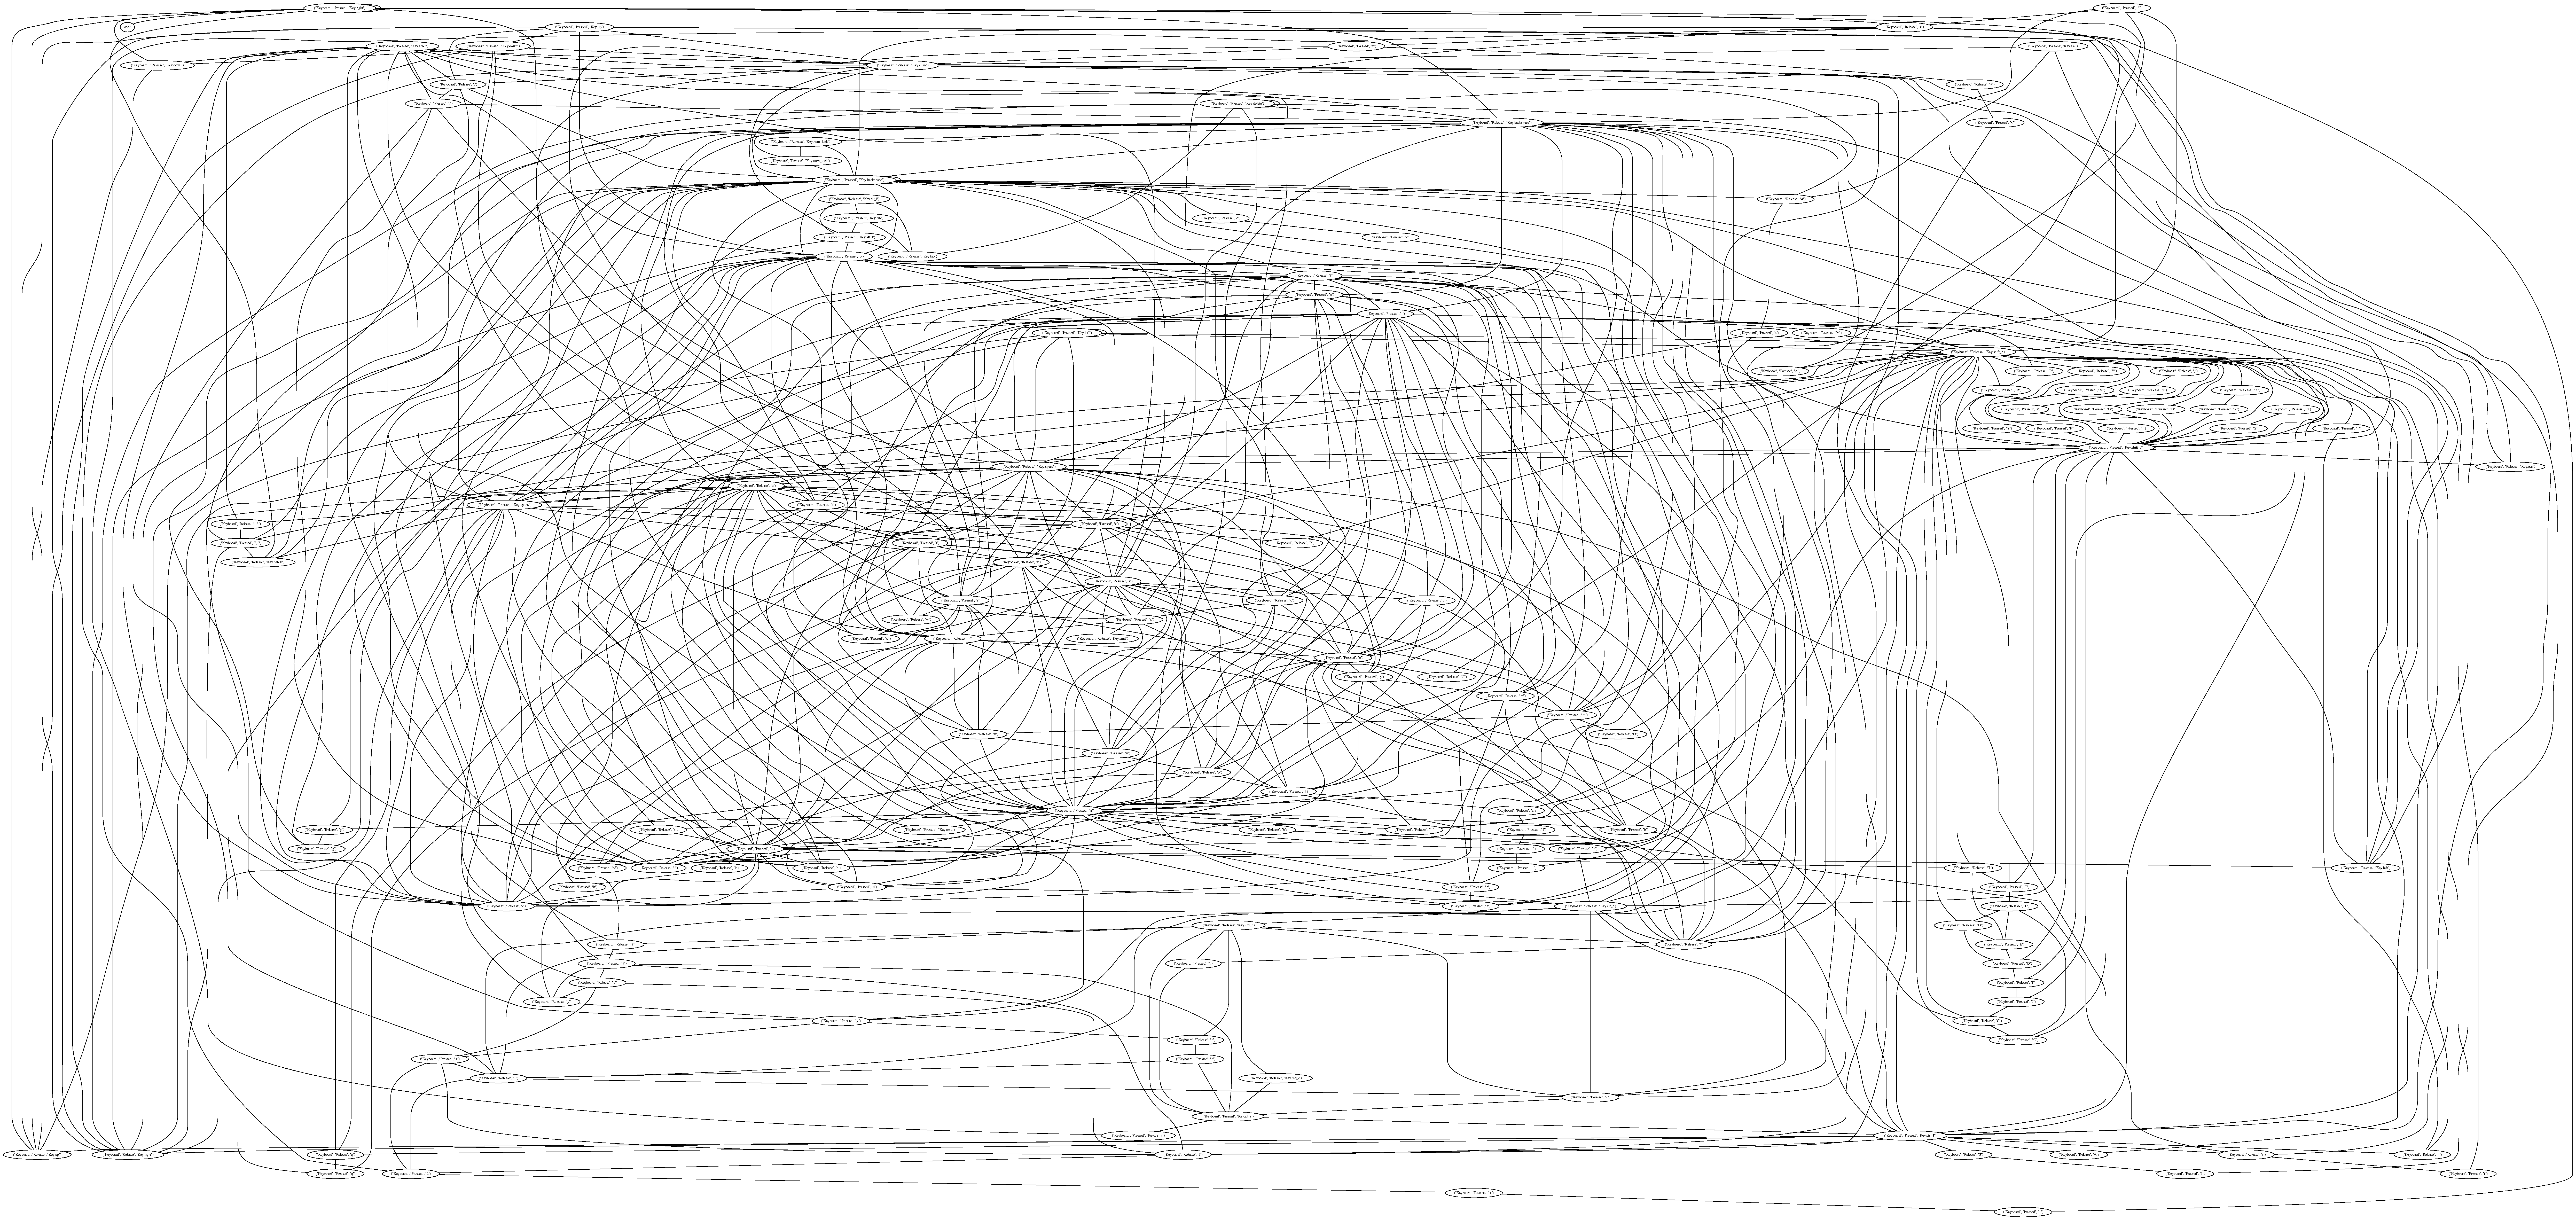
\includegraphics[width=1.0 \columnwidth]{chap5/Imagenes/GraphKB150.eps}
\caption{Grafo generado por el sujeto \emph{n\'umero 3} solo con acciones del 
 teclado.}
\label{fig:graphKB}
\end{figure}



\begin{figure}[h]
\centering
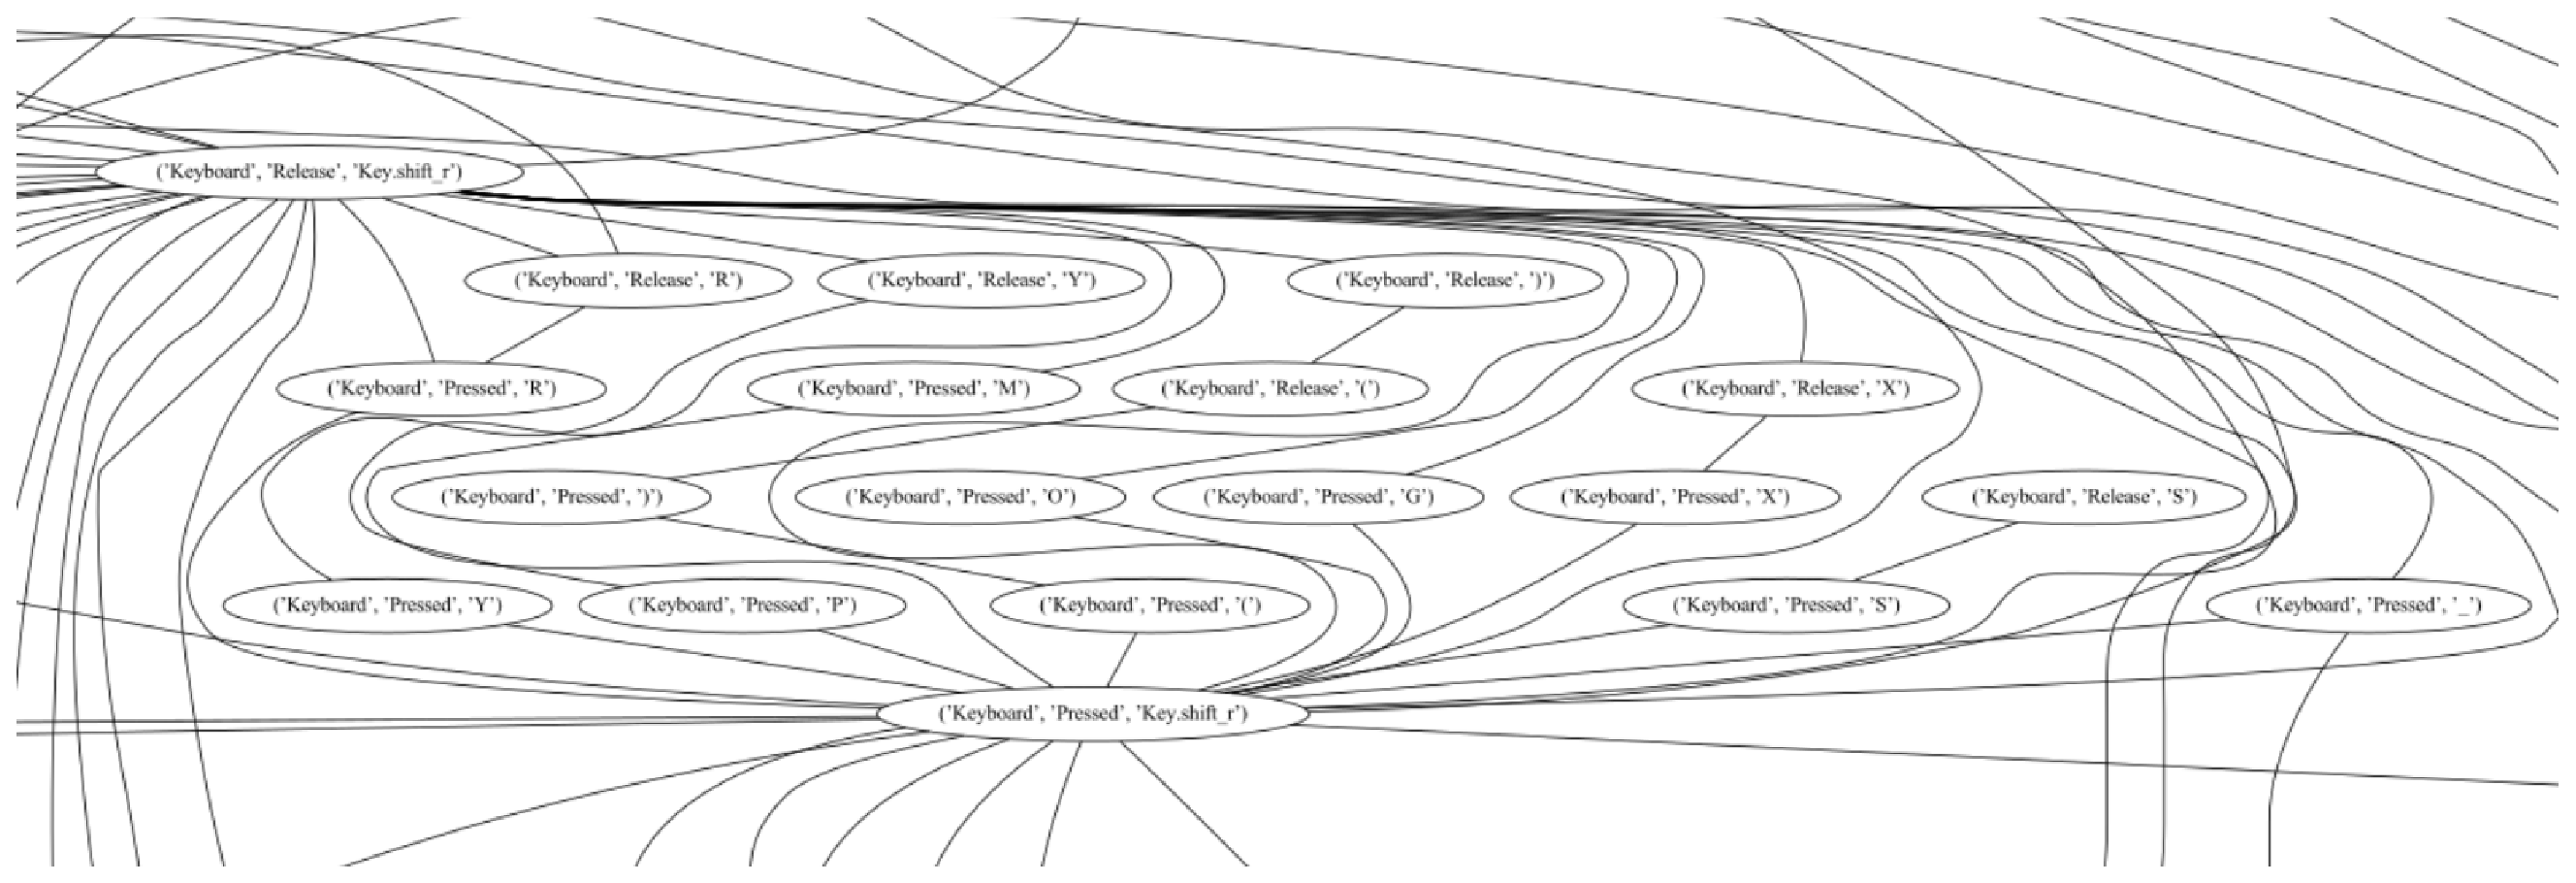
\includegraphics[width=1.0 \columnwidth]{chap5/Imagenes/ZoomKB150.eps}
\caption{Ampliaci\'on al grafo generado por el sujeto \emph{n\'umero 3} solo 
 con acciones del teclado.}
\label{fig:zoomKB}
\end{figure}


\begin{figure}[h]
\centering
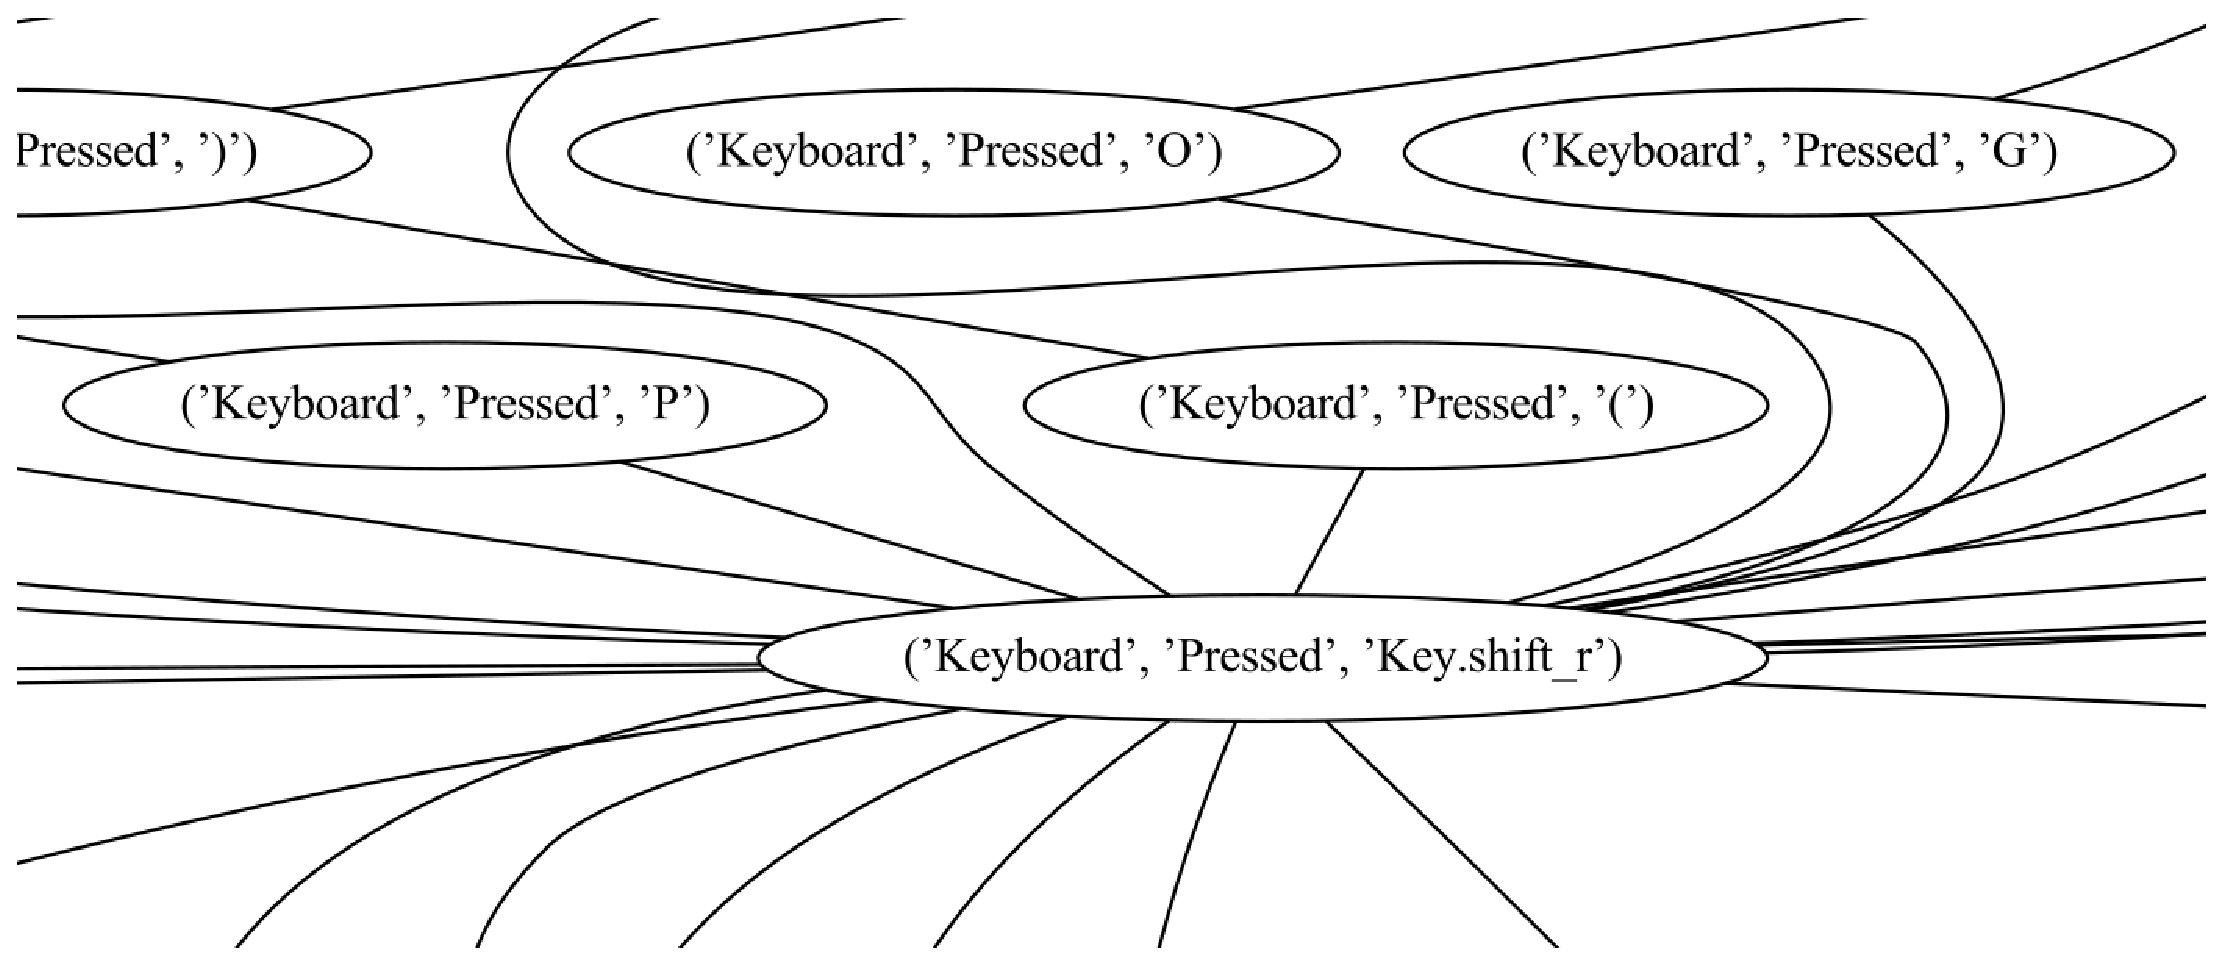
\includegraphics[width=1.0 \columnwidth]{chap5/Imagenes/MoreZKB150.eps}
\caption{Ampliaci\'on para la correcta visualizaci\'on de los nodos en el
 grafo generado por el sujeto \emph{n\'umero 3} solo con acciones del
 teclado.}
\label{fig:morezKB}
\end{figure}


Como filtro adicional, se limit\'o a obtener secuencias de 
 acciones con longitudes en m\'ultiplos de 2, considerando que una tecla o 
 bot\'on presionado debe de ser liberado para concluir la acci\'on, sin 
 embargo, pese a esta limitante, las secuencias a obtener naturalmente son; 
 desde una acci\'on (tabla \ref{tableRes1}) y desde dos acciones (tabla 
 \ref{tableRes2}). 
 

En la tabla \ref{tableRes1} cabe destacar que el sujeto \textbf{n\'umero 1}
 es al que se le detectaron mayor numero de secuencias y as\'i mismo es el 
 que tiene mayor n\'umero de \emph{Secuencias Aceptables} con el 36\% como
 \emph{Porcentaje de Precisi\'on}($P_P$), porcentaje obtenido de la ecuaci\'on
 \ref{eqAsertividad}, en la que se realiza la divici\'on de las 
 \emph{Secuencias Aceptables} ($S_A$) multiplicadas por $100$ entre el 
 \emph{Total de Secuencias Encontradas} ($S_T$); el sujeto \textbf{n\'umero 
 4} y \textbf{n\'umero 5} son los que obtuvieron menos \emph{Secuencias
 Aceptables} con un 31.11\%  y 34.64\% respectivamente de \emph{Porcentaje
 de Precisi\'on}.


\begin{equation}
P_P = \dfrac{ S_A \cdot 100}{S_T}
\label{eqAsertividad}
\end{equation}
 
 
En la tabla \ref{tableRes2} se observa que el sujeto \textbf{n\'umero 1} es 
 el que tiene mayor n\'umero de \emph{Secuencias Aceptables}, sin embargo, 
 es el que tiene el menor \emph{Porcentaje de Precisi\'on} con el 43.65\%, 
 mientras que el sujeto \textbf{n\'umero 5} es el que tiene la mayor
 \emph{precisi\'on} con el 45.37\%.


Por el hecho de que este es un m\'etodo de aprendizaje acumulativo, as\'i sea
 que la primer secuencia sea del agrado del usuario o no, la siguiente 
 secuencia puede contenerla con alguna acci\'on adicional y es mas 
 probable que esta variante, sea de utilidad al usuario. 

 
\begin{table}[]
\centering
\begin{tabular}{cccc}
\hline
\textbf{No. de }	
&	\textbf{Secuencias }	
&   \textbf{Secuencias }	
&	\textbf{Porcentaje de }	\\

\textbf{Sujeto}
&	\textbf{Aceptables}
&	\textbf{Totales}
&	\textbf{Precisi\'on}
	\\ \hline

1				
&	189						
&	525						
&	36.00 \%		\\

2				
&	165						
&	487						
&	33.88 \%		\\

3
&	151
&	467
&	32.33 \%		\\

4
&	56
&	180
&	31.11 \%		\\

5
&	53
&	153
&	34.64\%			\\
\hline
\end{tabular}
\caption{Tabla de resultados con secuencias de una longitud m\'inima de 
 1 acci\'on.}
\label{tableRes1}
\end{table}


\begin{table}[]
\centering
\begin{tabular}{cccc}
\hline
\textbf{No. de }	
&	\textbf{Secuencias }	
&   \textbf{Secuencias }	
&	\textbf{Porcentaje de }	\\

\textbf{Sujeto}
&	\textbf{Aceptables}
&	\textbf{Totales}
&	\textbf{Precisi\'on}
	\\ \hline

1
&	179
&	410
&	43.65 \%		\\
	
2
&	170
&	377
&	45.09 \%		\\

3
&	154
&	346
&	44.50 \%		\\

4
&	52
&	119
&	43.69 \%		\\

5
&	49
&	108
&	45.37\%			\\
\hline
\end{tabular}
\caption{Tabla de resultados con secuencias de una longitud m\'inima de 
 2 acciones.}
\label{tableRes2}
\end{table}

Recapitulando, para que una tarea sea identificable; los nodos que forman la
 secuencia deben de tener un m\'inimo de 75 repeticiones cada uno y cumplir 
 con las restricciones planteadas; no empezar con la acci\'on \emph{Release}, 
 no terminar con la acci\'on \emph{Pressed} y la longitud m\'inima de 
 2 acciones, por lo tanto, las secuencias mostradas a continuaci\'on
 cumplen con estas car\'acter\'isticas:
\\
\\
Sujeto: 1	\\
Descripci\'on: La tarea es utilizada en el software Blender para girar el 
 objeto en el eje Y.	\\
Secuencia obtenida:\\
Keyboard,Pressed,G\\
Keyboard,Release,G\\
Keyboard,Pressed,Y\\
Keyboard,Release,Y\\
\\
Sujeto: 2	\\
Descripci\'on: En Windows es utilizada esta combinaci\'on de teclas para 
 cambiar entre las ventanas abiertas.	\\
Secuencia obtenida:\\
Keyboard,Pressed,Key.alt\_l	\\
Keyboard,Pressed,Key.tab	\\
Keyboard,Release,Key.tab	\\
Keyboard,Release,Key.alt\_l	\\
\\
Sujeto: 3	\\
Descripci\'on: es la palabra ``el''.	\\
Secuencia obtenida:\\
Keyboard,Pressed,e	\\
Keyboard,Release,e	\\
Keyboard,Pressed,l	\\
Keyboard,Release,l	\\
\\
Sujeto: 4	\\
Descripci\'on: En Windows, selecciona el objeto se\~nalado por el puntero y
 obtiene el men\'u contextual de ese objeto.	\\
Secuencia obtenida:\\	
Mouse,Pressed,Button.left	\\
Mouse,Released,Button.left	\\
Mouse,Pressed,Button.right	\\
Mouse,Released,Button.right	\\
